\documentclass[11pt]{article}

\usepackage{lscape,color}
\usepackage{graphicx}

\topmargin -0.75truein
\oddsidemargin -0.4truein
\textheight 9.25truein
\textwidth 6.7truein
\hbadness=10001
\hfuzz=200pt


\begin{document}
%\input dspace12.tex
%\input pstricks.tex
%\input psfig
\newcommand{\be}{\begin{enumerate}}
\newcommand{\ee}{\end{enumerate}}
\newcommand{\bc}{\begin{center}}
\newcommand{\ec}{\end{center}}
\newcommand{\bi}{\begin{itemize}}
\newcommand{\ei}{\end{itemize}}
\newcommand{\bd}{\begin{description}}
\newcommand{\ed}{\end{description}}
\newcommand{\bt}{\begin{tabbing}}
\newcommand{\et}{\end{tabbing}}
\newcommand{\eg}{{\it e.g.~}}
\newcommand{\ie}{{\it i.e.~}}
\newcommand{\ul}{\underline}
\newcommand{\axaf}{{\em AXAF}}
\def\la{\hbox{\rlap{$<$}\lower0.5ex\hbox{$\sim$}\ }}


\large
%\vspace*{-0.5in}
\centerline {\bf 4.29\_V2.2 TURN ON DEA A AND TEST VIDEO BOARDS }
\vspace{0.25in}

\normalsize
\noindent{\it Last Revised: October 2, 2017}\\
\noindent{\bf Filename: deaa\_on\_test\_vid} \\


\noindent {\bf BRIEF FUNCTIONAL DESCRIPTION:} \\
\normalsize

This is a procedure which powers up the DEA side A, powers up all 10 video boards, and powers up all 6 FEPs. It then executes an ACIS-I bias-only science run and an ACIS-S bias-only science run in order to get calibrated housekeeping data from the video boards. It then powers down all video boards and FEPs. It should be safe to execute under any condition except a spacecraft power or thermal emergency.

\vspace{0.25in}
\noindent The sequence of actions for this procedure will be:
\be
\item Verify that DEA B is powered off and disabled (see Constraints/Cautions, below)
\vspace{-0.10in}
\item Verify that DEA A is receiving power from the spacecraft
\vspace{-0.10in}
\item Enable and turn on DEA power supply side A
\vspace{-0.10in}
\item Verify that DEA B is still off
\vspace{-0.10in}
\item Verify that the DH heater is not powered from side A
\vspace{-0.10in}
\item Warm boot the BEP
\vspace{-0.10in}
\item Execute a DEA housekeeping run
\vspace{-0.10in}
\item Set the focal plane temperature to -119.7~$^\circ$C
\vspace{-0.10in}
\item Power up all 10 video boards
\vspace{-0.10in}
\item Execute an ACIS-I bias-only science run to capture calibrated video housekeeping data
\vspace{-0.10in}
\item Execute an ACIS-S bias-only science run to capture calibrated video housekeeping data
\vspace{-0.10in}
\item Power down the 10 video boards and the 6 FEPs
\ee

\vspace{0.15in}
\normalsize
\noindent {\bf ASSUMED INSTRUMENT STATE:} \\
\normalsize
\be
\item Assumes that the PSMC has power from the spacecraft.
\vspace{-0.10in}
\item Assumes that DEA B is off.
\vspace{-0.10in}
\item Assumes that both sides of the DPA are on.
\vspace{-0.10in}
\item Assumes that the DEA was previously powered from side A. 
If it was instead powered from side B, the board 11 relays must be reset in
addition to powering on DEA A.
\ee
\vspace{0.1in}
%\vspace{0.25in}
\normalsize
\noindent {\bf SPECIAL INITIAL CONDITIONS:} \\
\normalsize

\normalsize
\noindent {\bf OPERATIONAL CONSTRAINTS/CAUTIONS:} \\
\normalsize

In normal operations, only one side of the DEA should be powered on
(a) to prevent conflict for control of the focal plane temperature controller,
(b) to avoid excess current draw from the spacecraft,(c) to avoid over-heating
within the PSMC, and (d) to avoid placing a board 11 relay into the 
``magnetic neutral position''.

The DEA power status is normally indicated by the values of the 1DEPSA and
1DEPSB flags, which should not both be 1 simultaneously. Before sending the 
command to power on DEA A, the DEA Input Voltage A 1DE28AVO should 
be checked to make sure that DEA A is receiving power from the spacecraft.

The DEA input current monitors (1DEIC[AB]CU) are noisy.
To give an indication of what variation may be expected, figures 1 and 2
show the behavior of the A-side DEA current with a ten-sample running
average for two situations in which all video boards were powered down. Note that
when either side of the DEA is unpowered, the corresponding current monitor, 
1DEICACU for side A, or 1DEICBCU for side B, will be unreliable. They will read
16--18~A when unpowered, as of Telemetry Database (TDB) v14. This is expected and
not a problem.

If the DEA powers off unexpectedly during a bakeout, the FP bakeout 
heater will lose power and this heater will NOT be re-enabled when the DEA side A 
power is restored. Additional SW commands are necessary to activate the FP bakeout 
heater. The DH bakeout heater is unaffected by a power loss to the DEA and will 
therefore still be executing a bakeout if power is lost to the DEA.

The parameters for the threshold crossings patch, txings, will revert to defaults 
when this is run. They should be restored to their desired values.

After successful execution, {\em the FP temperature control will be regulated at 
-119.7~$^\circ$C (if the spacecraft thermal environment allows), and DEA interface 
A/D will be in high-resolution mode.}\\

\vspace{0.15in}
\normalsize
\noindent {\bf REFERENCES:} \\
\normalsize

\normalsize
\noindent {\bf CHANGE HISTORY:} \\
\normalsize

{\bf V2.0}
\begin{itemize}
\item Branched off from ``deaa\_on'' atomic procedure V2.2
\item Add commands to power video boards on and off
\item Add bias-only science runs
\end{itemize}

{\bf V2.1}
\begin{itemize}
\item Added a step to verify DEA-B is off at the beginning of the procedure
\item Added text regarding power status issues and expected current behavior to the Operational Constraints/Cautions section. Also updated the expected FP temperature control.
\item Removed language about what to do if the DPA is unpowered since we do not expect to run this procedure if that is the case.
\item Removed input current check for DEA B; added warning to text.
\item Corrected introduction to indicate that we will be powering down all video boards and all FEPs at the end
\item Corrected numbering in table: 5.2 $\rightarrow$ 6.2
\item Corrected number of FEPMAN\_POWEROFF messages in Step 6.1 of the table
\end{itemize}

{\bf V2.2}
\begin{itemize}
\item Added a step to verify that the DEA is being powered from the spacecraft
\item Added a step to warmboot the BEP after powering on DEA-A
\item Added a step to execute a DEA housekeeping run after warmbooting the BEP
\item Added a step to set the focal plane temperature after the DEA housekeeping run
\item Added comments about what will happen to the bakeout heaters if the DEA powers off during a bakeout
\item Noted that after this procedure the DEA interface A/D will be in high-resolution mode. 
\item Added a note that this procedure assumes that the DEA was powered from side A and what to do if it was not
\end{itemize}

\begin{landscape}
\begin{figure}
\begin{center}
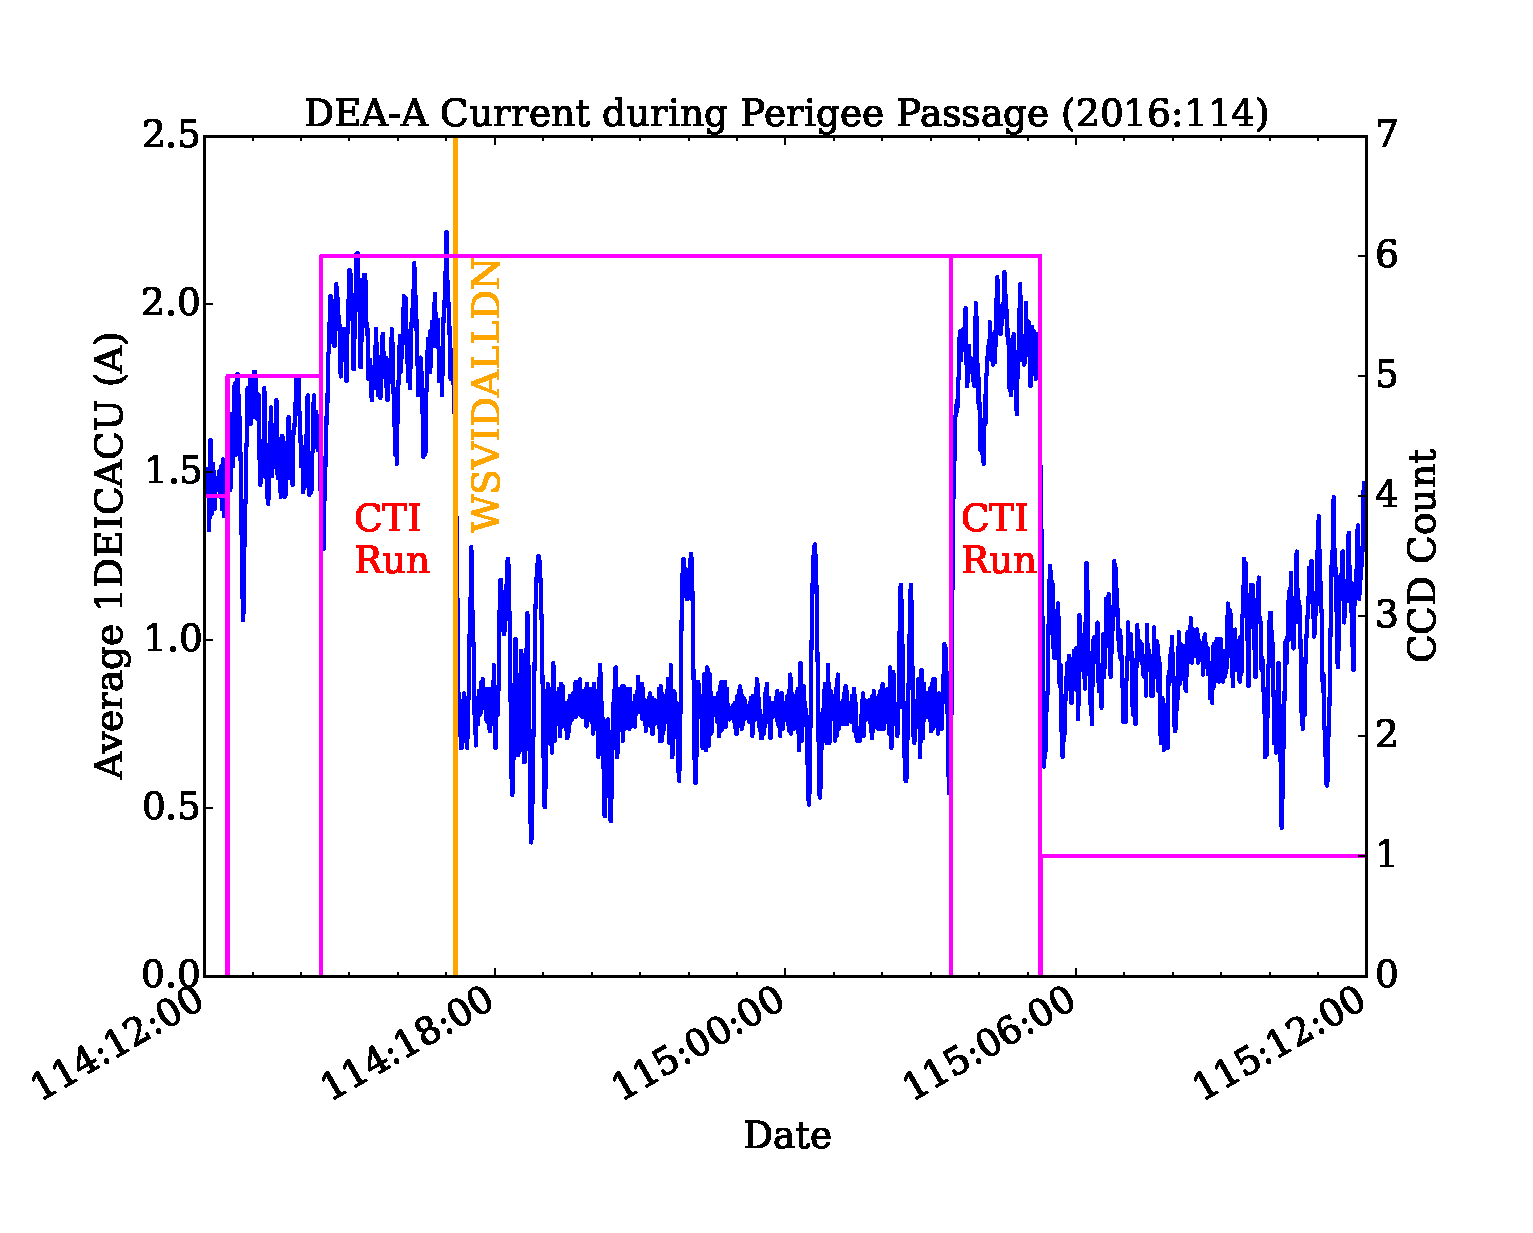
\includegraphics[width=1.2\textwidth]{deaa_on_test_vid_fig1.eps}
\caption{Average behavior of 1DEICACU during a perigee passage. All video boards
are powered off after the issuing of the WSVIDALLDN command, which is marked by
the orange line in the plot.}
\end{center}
\end{figure}
\end{landscape}

\begin{landscape}
\begin{figure}
\begin{center}
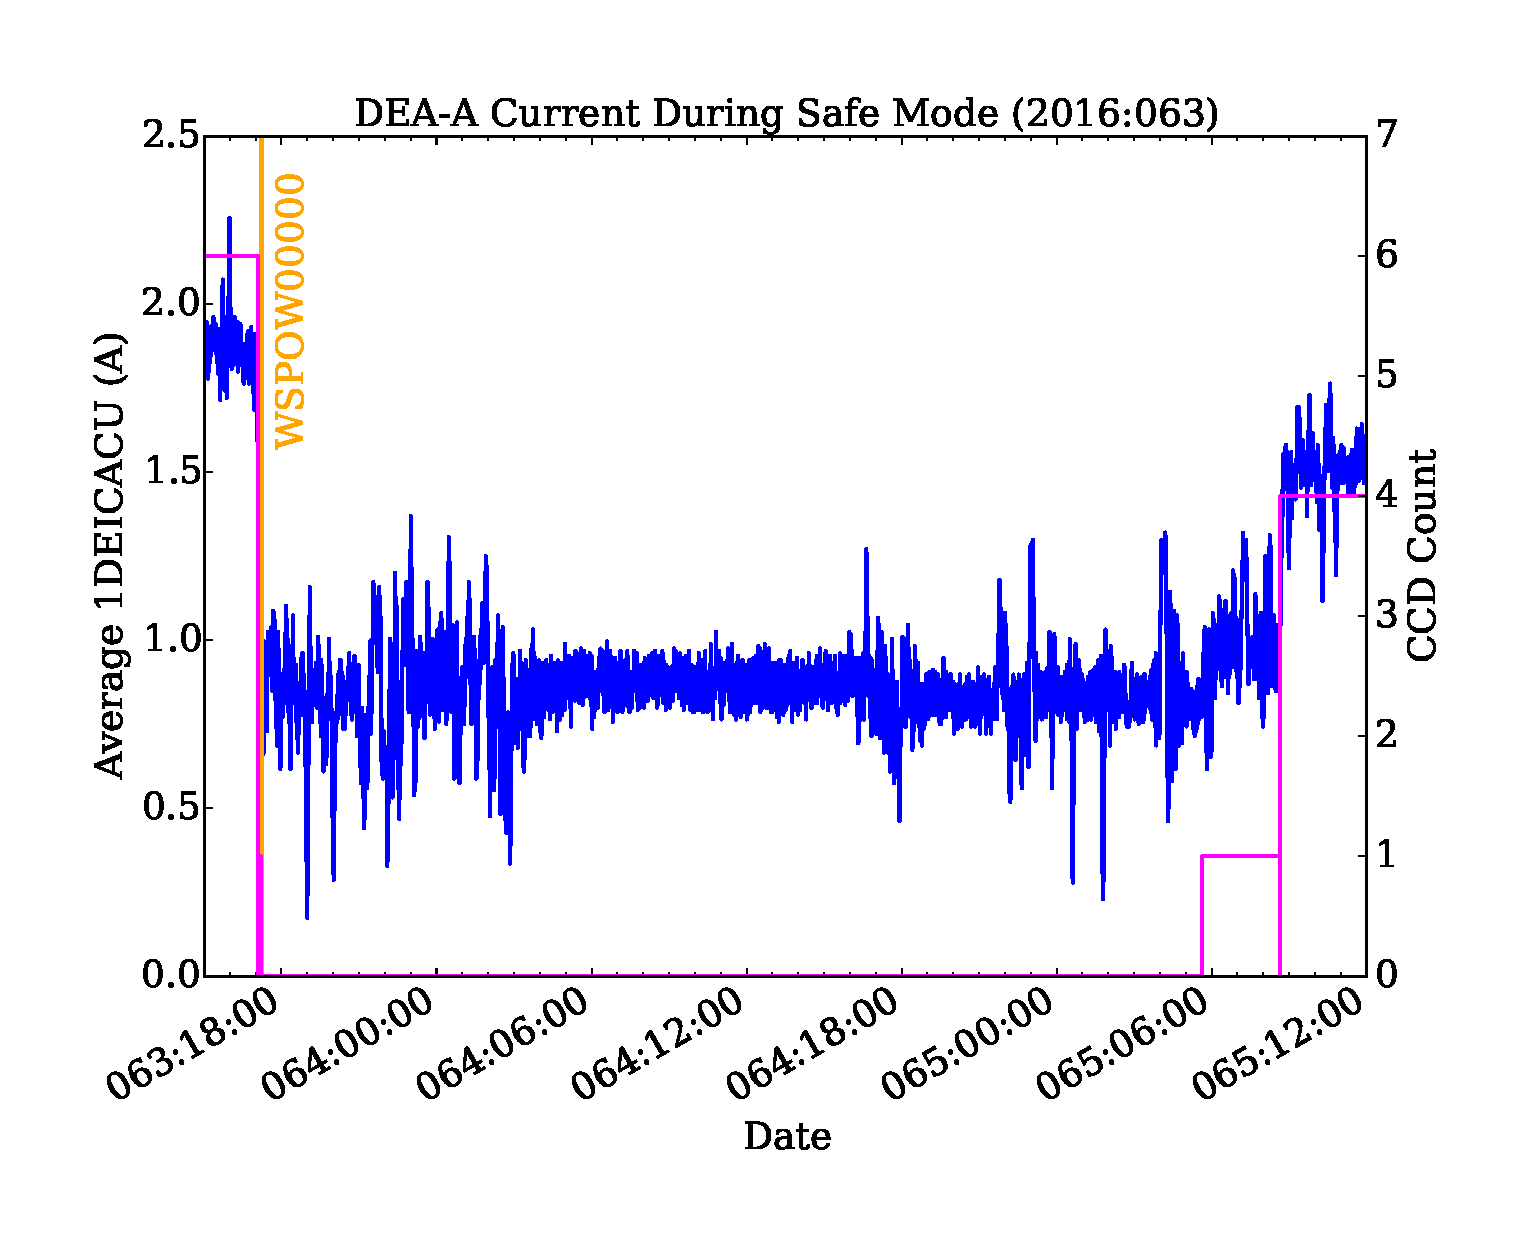
\includegraphics[width=1.2\textwidth]{deaa_on_test_vid_fig2.eps}
\caption{Average behavior of 1DEICACU during a safe mode. All video boards
are powered off after the issuing of the WSPOW00000 command, which is marked by
the orange line in the plot.}
\end{center}
\end{figure}
\end{landscape}

\begin{landscape}
\begin{figure}
\begin{center}
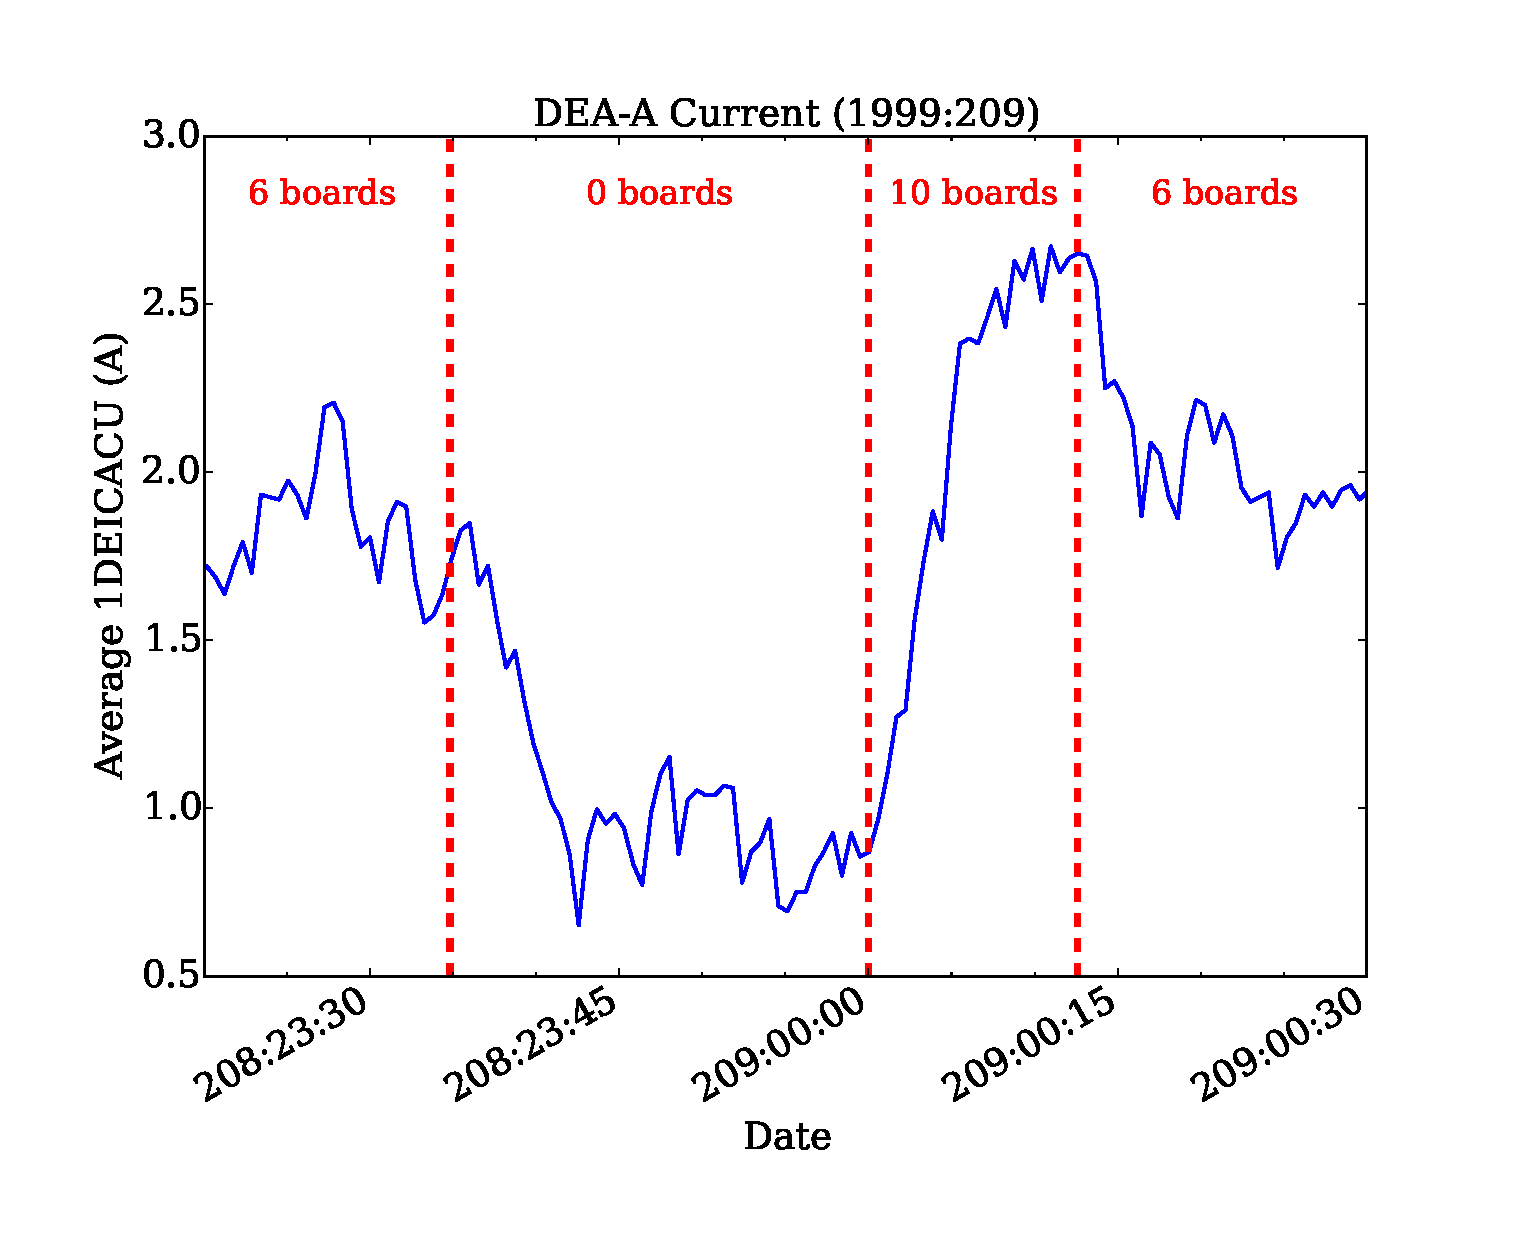
\includegraphics[width=1.2\textwidth]{deaa_on_test_vid_fig3.eps}
\caption{Average behavior of 1DEICACU with different numbers of video boards
powered on. The plot is a 10-sample running average of the current readings.}
\end{center}
\end{figure}
\end{landscape}

\newpage\
\vspace{0.4\textheight}
\bc This page is intentionally blank \ec

\newcommand{\tablecaptiontext}{TURN ON DEA A AND TEST VIDEO BOARDS}
\documentclass[11pt]{article}

\usepackage{lscape,color}
\usepackage{graphicx}

\topmargin -0.75truein
\oddsidemargin -0.4truein
\textheight 9.25truein
\textwidth 6.7truein
\hbadness=10001
\hfuzz=200pt


\begin{document}
%\input dspace12.tex
%\input pstricks.tex
%\input psfig
\newcommand{\be}{\begin{enumerate}}
\newcommand{\ee}{\end{enumerate}}
\newcommand{\bc}{\begin{center}}
\newcommand{\ec}{\end{center}}
\newcommand{\bi}{\begin{itemize}}
\newcommand{\ei}{\end{itemize}}
\newcommand{\bd}{\begin{description}}
\newcommand{\ed}{\end{description}}
\newcommand{\bt}{\begin{tabbing}}
\newcommand{\et}{\end{tabbing}}
\newcommand{\eg}{{\it e.g.~}}
\newcommand{\ie}{{\it i.e.~}}
\newcommand{\ul}{\underline}
\newcommand{\axaf}{{\em AXAF}}
\def\la{\hbox{\rlap{$<$}\lower0.5ex\hbox{$\sim$}\ }}


\large
%\vspace*{-0.5in}
\centerline {\bf 4.29\_V2.1 TURN ON DEA A AND TEST VIDEO BOARDS }
\vspace{0.25in}

\normalsize
\noindent{\it Last Revised: June 5, 2017}\\
\noindent{\bf Filename: deaa\_on\_test\_vid} \\


\noindent {\bf BRIEF FUNCTIONAL DESCRIPTION:} \\
\normalsize

This is a procedure which powers up the DEA side A, powers up all 10 video boards, and powers up all 6 FEPs. It then executes an ACIS-I bias-only science run and an ACIS-S bias-only science run in order to get calibrated housekeeping data from the video boards. It then powers down all video boards and FEPs. It should be safe to execute under any condition except a spacecraft power or thermal emergency.

\vspace{0.25in}
\noindent The sequence of actions for this procedure will be:
\be
\item Verify that DEA B is powered off and disabled (see Constraints/Cautions, below)
\vspace{-0.10in}
\item Enable and turn on DEA power supply side A
\vspace{-0.10in}
\item Verify that DEA B is still off
\vspace{-0.10in}
\item Verify that the DH heater is not powered from side A
\vspace{-0.10in}
\item Power up all 10 video boards
\vspace{-0.10in}
\item Execute two bias-only science runs to capture video housekeeping
\vspace{-0.10in}
\item Power down the 10 video boards and the 6 FEPs
\ee

\vspace{0.15in}
\normalsize
\noindent {\bf ASSUMED INSTRUMENT STATE:} \\
\normalsize
\be
\item Assumes that the PSMC has power from the spacecraft.
\vspace{-0.10in}
\item Assumes that DEA B is off.
\vspace{-0.10in}
\item Assumes that both sides of the DPA are on.
\vspace{-0.10in}
\item Assumes that the flight SW is running on the active BEP.
\ee
\vspace{0.1in}
%\vspace{0.25in}
\normalsize
\noindent {\bf SPECIAL INITIAL CONDITIONS:} \\
\normalsize
%The environment must be clean enough to allow opening of the valve. \\
%Assumes that \axaf\/ ISIM RCTU is powered on and in telemetry format 6. \\

%\vspace{0.25in}
\normalsize
\noindent {\bf OPERATIONAL CONSTRAINTS/CAUTIONS:} \\
\normalsize

In normal operations, only one side of the DEA should be powered on
(a) to prevent conflict for control of the focal plane temperature controller,
(b) to avoid excess current draw from the spacecraft, and (c) to avoid over-heating
within the PSMC.

The DEA power status is normally indicated by the values of the 1DEPSA and
1DEPSB flags, which should not both be 1 simultaneously.

The DEA input current monitors (1DEIC[AB]CU) are noisy.
To give an indication of what variation may be expected, figures 1 and 2
show the behavior of the A-side DEA current with a ten-sample running
average for two situations in which all video boards were powered down. Note that
when either side of the DEA is unpowered, the corresponding current monitor, 
1DEICACU for side A, or 1DEICBCU for side B, will be unreliable. They will read
16--18~A when unpowered, as of Telemetry Database (TDB) v14. This is expected and
not a problem.

After successful execution, {\em the FP temperature control will be unregulated,
and DEA interface A/D will be in low-resolution mode.}\\

\vspace{0.15in}
\normalsize
\noindent {\bf REFERENCES:} \\
\normalsize

\normalsize
\noindent {\bf CHANGE HISTORY:} \\
\normalsize

{\bf V2.0}
\begin{itemize}
\item Branched off from ``deaa\_on'' atomic procedure V2.2
\item Add commands to power video boards on and off
\item Add bias-only science runs
\end{itemize}

{\bf V2.1}
\begin{itemize}
\item Added a step to verify DEA-B is off at the beginning of the procedure
\item Added text regarding power status issues and expected current behavior to the Operational Constraints/Cautions section. Also updated the expected FP temperature control.
\item Removed language about what to do if the DPA is unpowered since we do not expect to run this procedure if that is the case.
\item Removed input current check for DEA B; added warning to text.
\item Corrected introduction to indicate that we will be powering down all video boards and all FEPs at the end
\item Corrected numbering in table: 5.2 $\rightarrow$ 6.2
\item Corrected number of FEPMAN\_POWEROFF messages in Step 6.1 of the table
\end{itemize}

\begin{landscape}
\begin{figure}
\begin{center}
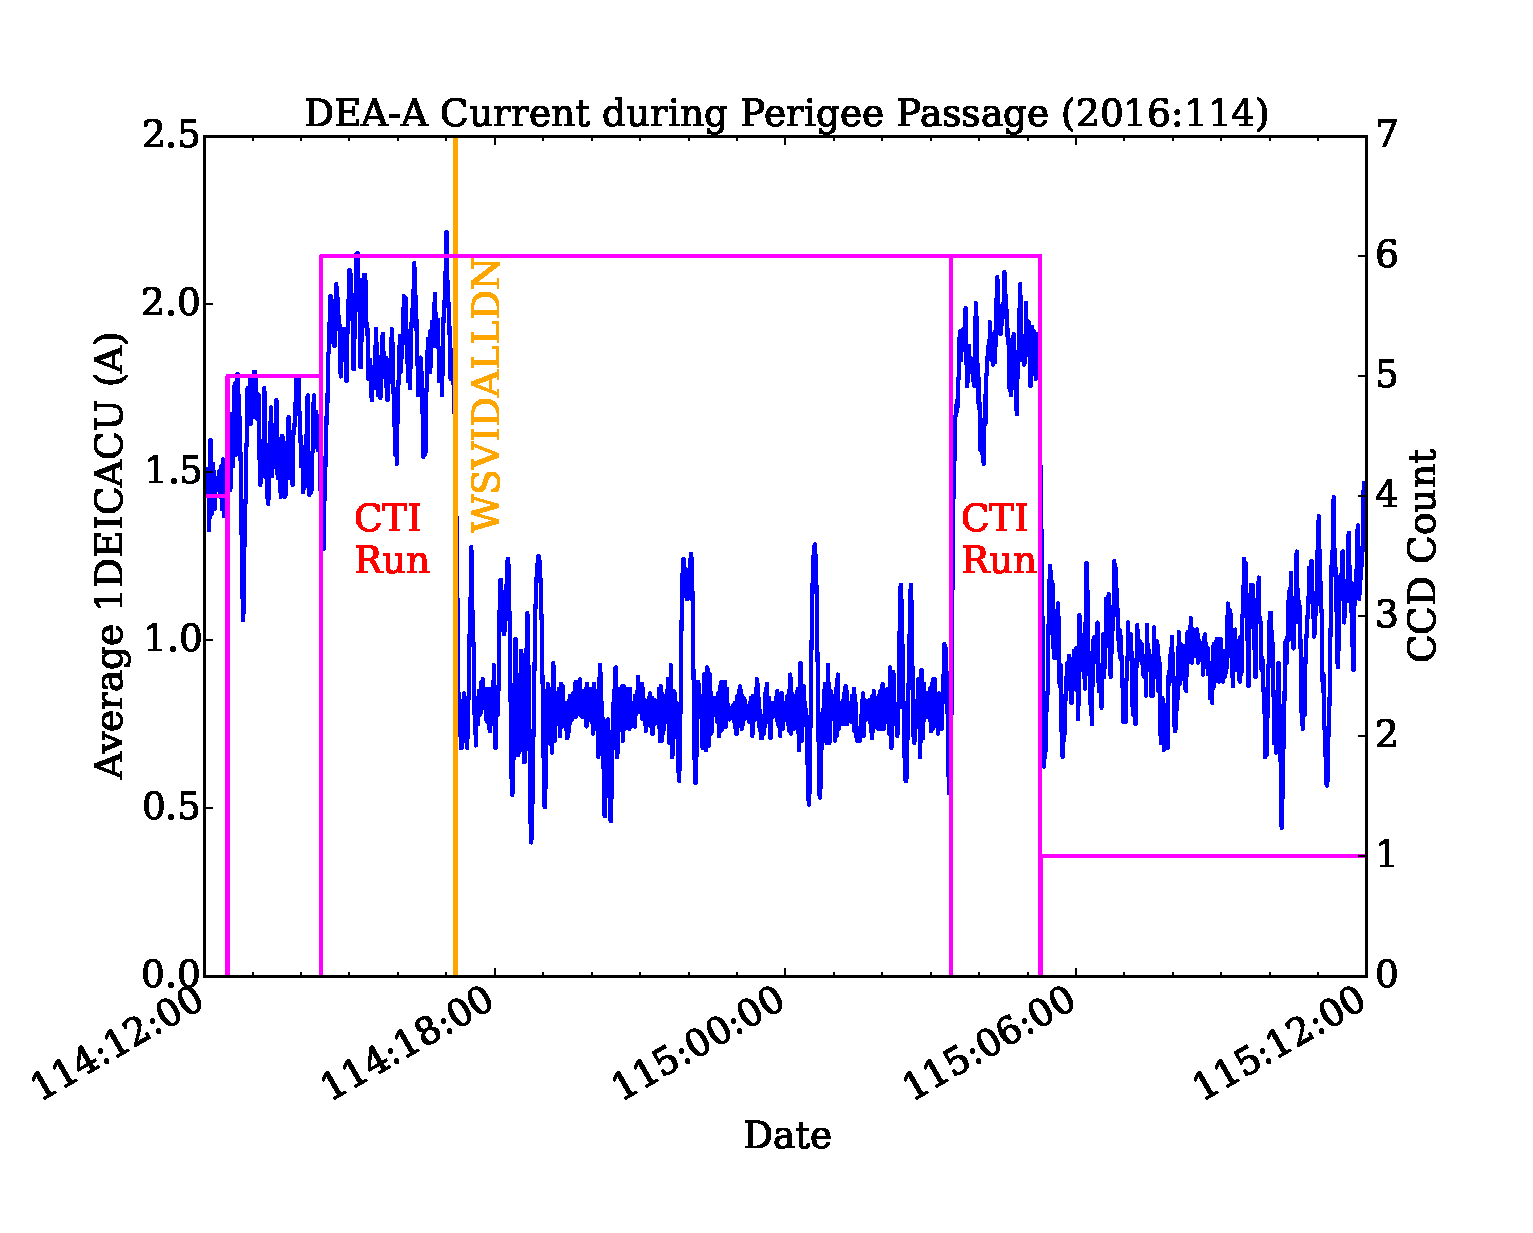
\includegraphics[width=1.2\textwidth]{deaa_on_test_vid_fig1.eps}
\caption{Average behavior of 1DEICACU during a perigee passage. All video boards
are powered off after the issuing of the WSVIDALLDN command, which is marked by
the orange line in the plot.}
\end{center}
\end{figure}
\end{landscape}

\begin{landscape}
\begin{figure}
\begin{center}
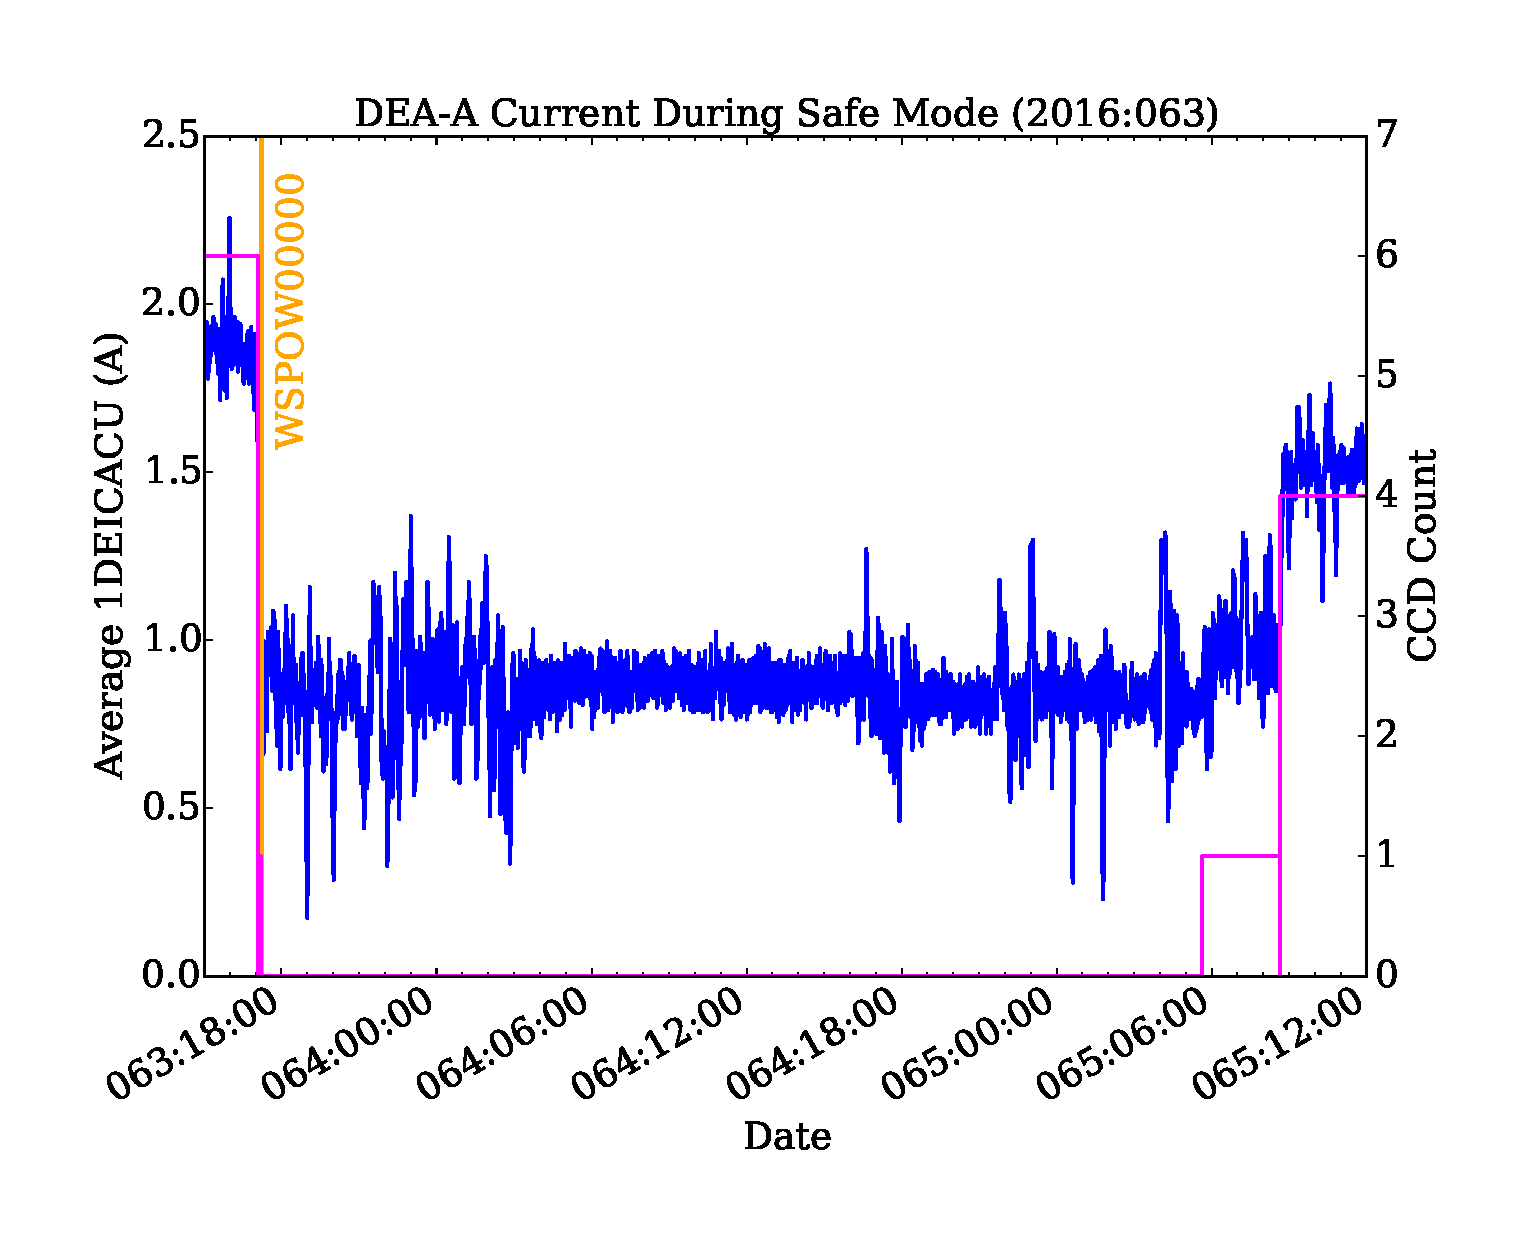
\includegraphics[width=1.2\textwidth]{deaa_on_test_vid_fig2.eps}
\caption{Average behavior of 1DEICACU during a safe mode. All video boards
are powered off after the issuing of the WSPOW00000 command, which is marked by
the orange line in the plot.}
\end{center}
\end{figure}
\end{landscape}

\begin{landscape}
\begin{figure}
\begin{center}
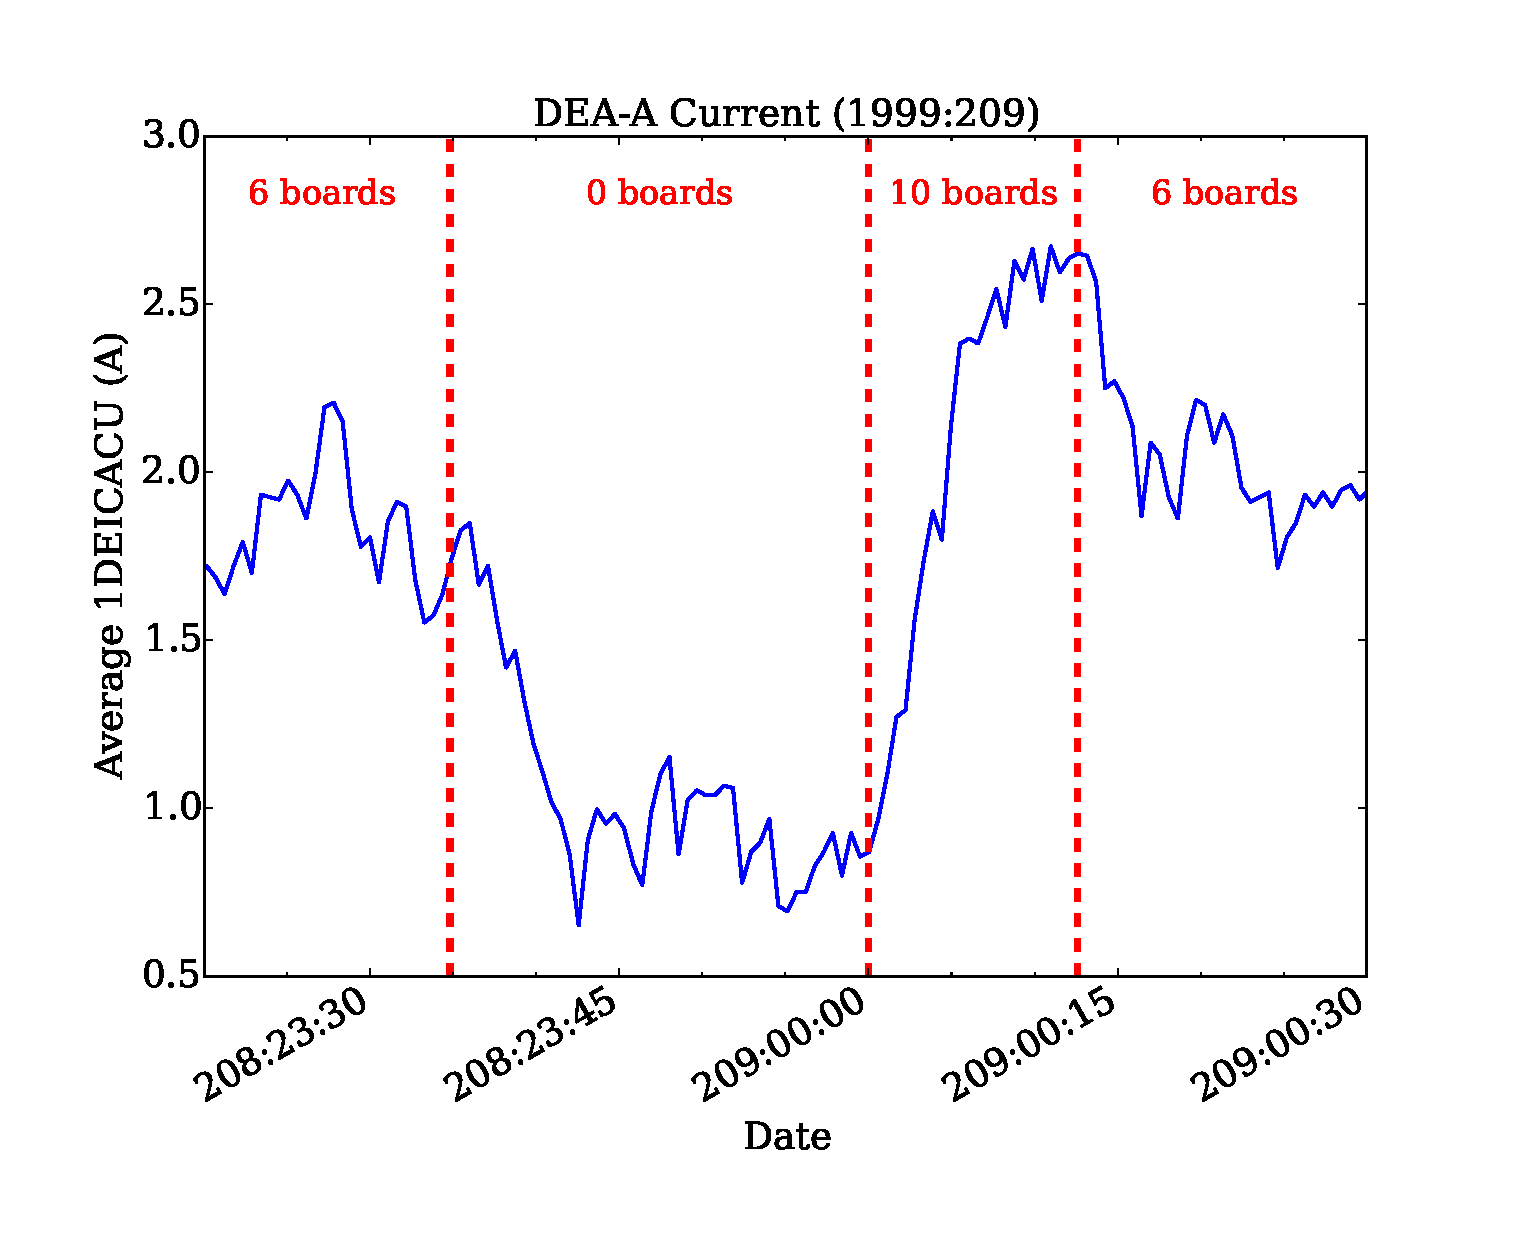
\includegraphics[width=1.2\textwidth]{deaa_on_test_vid_fig3.eps}
\caption{Average behavior of 1DEICACU with different numbers of video boards
powered on.}
\end{center}
\end{figure}
\end{landscape}

%\newpage\
%\vspace{0.4\textheight}
%\bc This page is intentionally blank \ec

\newcommand{\tablecaptiontext}{TURN ON DEA A AND TEST VIDEO BOARDS}
\documentclass[11pt]{article}

\usepackage{lscape,color}
\usepackage{graphicx}

\topmargin -0.75truein
\oddsidemargin -0.4truein
\textheight 9.25truein
\textwidth 6.7truein
\hbadness=10001
\hfuzz=200pt


\begin{document}
%\input dspace12.tex
%\input pstricks.tex
%\input psfig
\newcommand{\be}{\begin{enumerate}}
\newcommand{\ee}{\end{enumerate}}
\newcommand{\bc}{\begin{center}}
\newcommand{\ec}{\end{center}}
\newcommand{\bi}{\begin{itemize}}
\newcommand{\ei}{\end{itemize}}
\newcommand{\bd}{\begin{description}}
\newcommand{\ed}{\end{description}}
\newcommand{\bt}{\begin{tabbing}}
\newcommand{\et}{\end{tabbing}}
\newcommand{\eg}{{\it e.g.~}}
\newcommand{\ie}{{\it i.e.~}}
\newcommand{\ul}{\underline}
\newcommand{\axaf}{{\em AXAF}}
\def\la{\hbox{\rlap{$<$}\lower0.5ex\hbox{$\sim$}\ }}


\large
%\vspace*{-0.5in}
\centerline {\bf 4.29\_V2.1 TURN ON DEA A AND TEST VIDEO BOARDS }
\vspace{0.25in}

\normalsize
\noindent{\it Last Revised: June 5, 2017}\\
\noindent{\bf Filename: deaa\_on\_test\_vid} \\


\noindent {\bf BRIEF FUNCTIONAL DESCRIPTION:} \\
\normalsize

This is a procedure which powers up the DEA side A, powers up all 10 video boards, and powers up all 6 FEPs. It then executes an ACIS-I bias-only science run and an ACIS-S bias-only science run in order to get calibrated housekeeping data from the video boards. It then powers down all video boards and FEPs. It should be safe to execute under any condition except a spacecraft power or thermal emergency.

\vspace{0.25in}
\noindent The sequence of actions for this procedure will be:
\be
\item Verify that DEA B is powered off and disabled (see Constraints/Cautions, below)
\vspace{-0.10in}
\item Enable and turn on DEA power supply side A
\vspace{-0.10in}
\item Verify that DEA B is still off
\vspace{-0.10in}
\item Verify that the DH heater is not powered from side A
\vspace{-0.10in}
\item Power up all 10 video boards
\vspace{-0.10in}
\item Execute two bias-only science runs to capture video housekeeping
\vspace{-0.10in}
\item Power down the 10 video boards and the 6 FEPs
\ee

\vspace{0.15in}
\normalsize
\noindent {\bf ASSUMED INSTRUMENT STATE:} \\
\normalsize
\be
\item Assumes that the PSMC has power from the spacecraft.
\vspace{-0.10in}
\item Assumes that DEA B is off.
\vspace{-0.10in}
\item Assumes that both sides of the DPA are on.
\vspace{-0.10in}
\item Assumes that the flight SW is running on the active BEP.
\ee
\vspace{0.1in}
%\vspace{0.25in}
\normalsize
\noindent {\bf SPECIAL INITIAL CONDITIONS:} \\
\normalsize
%The environment must be clean enough to allow opening of the valve. \\
%Assumes that \axaf\/ ISIM RCTU is powered on and in telemetry format 6. \\

%\vspace{0.25in}
\normalsize
\noindent {\bf OPERATIONAL CONSTRAINTS/CAUTIONS:} \\
\normalsize

In normal operations, only one side of the DEA should be powered on
(a) to prevent conflict for control of the focal plane temperature controller,
(b) to avoid excess current draw from the spacecraft, and (c) to avoid over-heating
within the PSMC.

The DEA power status is normally indicated by the values of the 1DEPSA and
1DEPSB flags, which should not both be 1 simultaneously.

The DEA input current monitors (1DEIC[AB]CU) are noisy.
To give an indication of what variation may be expected, figures 1 and 2
show the behavior of the A-side DEA current with a ten-sample running
average for two situations in which all video boards were powered down. Note that
when either side of the DEA is unpowered, the corresponding current monitor, 
1DEICACU for side A, or 1DEICBCU for side B, will be unreliable. They will read
16--18~A when unpowered, as of Telemetry Database (TDB) v14. This is expected and
not a problem.

After successful execution, {\em the FP temperature control will be unregulated,
and DEA interface A/D will be in low-resolution mode.}\\

\vspace{0.15in}
\normalsize
\noindent {\bf REFERENCES:} \\
\normalsize

\normalsize
\noindent {\bf CHANGE HISTORY:} \\
\normalsize

{\bf V2.0}
\begin{itemize}
\item Branched off from ``deaa\_on'' atomic procedure V2.2
\item Add commands to power video boards on and off
\item Add bias-only science runs
\end{itemize}

{\bf V2.1}
\begin{itemize}
\item Added a step to verify DEA-B is off at the beginning of the procedure
\item Added text regarding power status issues and expected current behavior to the Operational Constraints/Cautions section. Also updated the expected FP temperature control.
\item Removed language about what to do if the DPA is unpowered since we do not expect to run this procedure if that is the case.
\item Removed input current check for DEA B; added warning to text.
\item Corrected introduction to indicate that we will be powering down all video boards and all FEPs at the end
\item Corrected numbering in table: 5.2 $\rightarrow$ 6.2
\item Corrected number of FEPMAN\_POWEROFF messages in Step 6.1 of the table
\end{itemize}

\begin{landscape}
\begin{figure}
\begin{center}
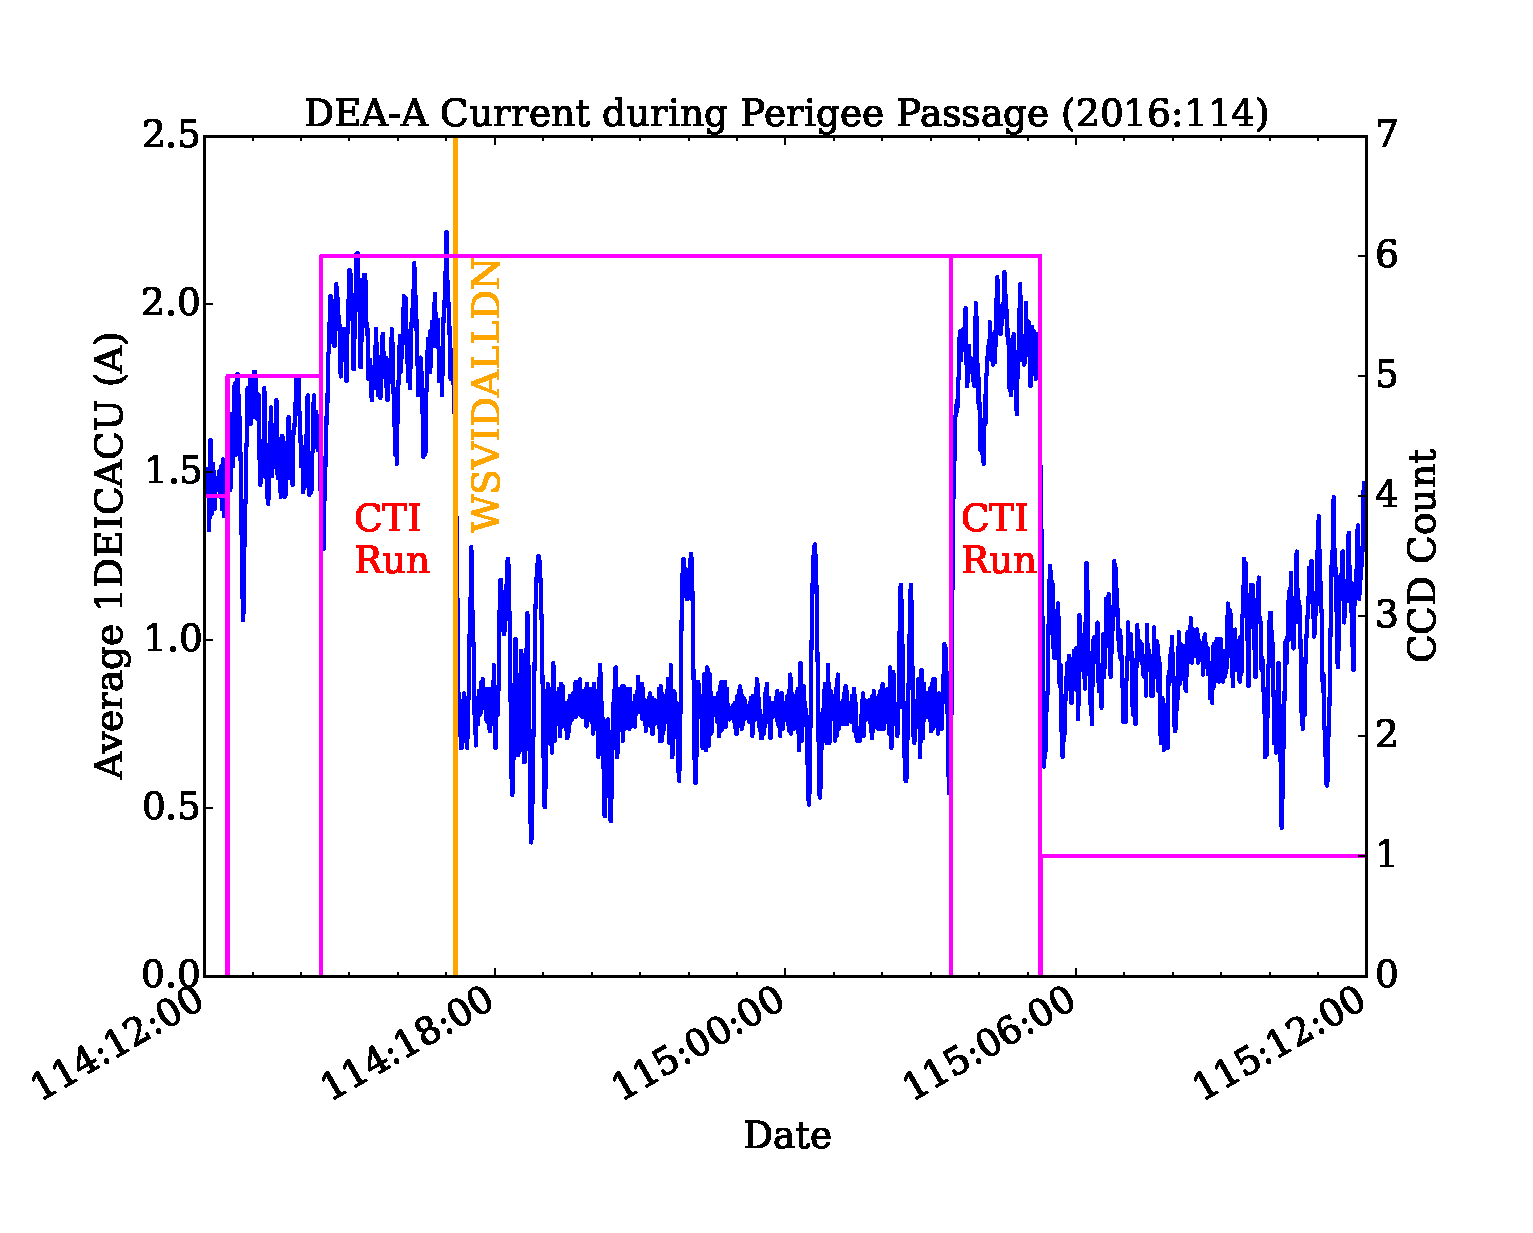
\includegraphics[width=1.2\textwidth]{deaa_on_test_vid_fig1.eps}
\caption{Average behavior of 1DEICACU during a perigee passage. All video boards
are powered off after the issuing of the WSVIDALLDN command, which is marked by
the orange line in the plot.}
\end{center}
\end{figure}
\end{landscape}

\begin{landscape}
\begin{figure}
\begin{center}
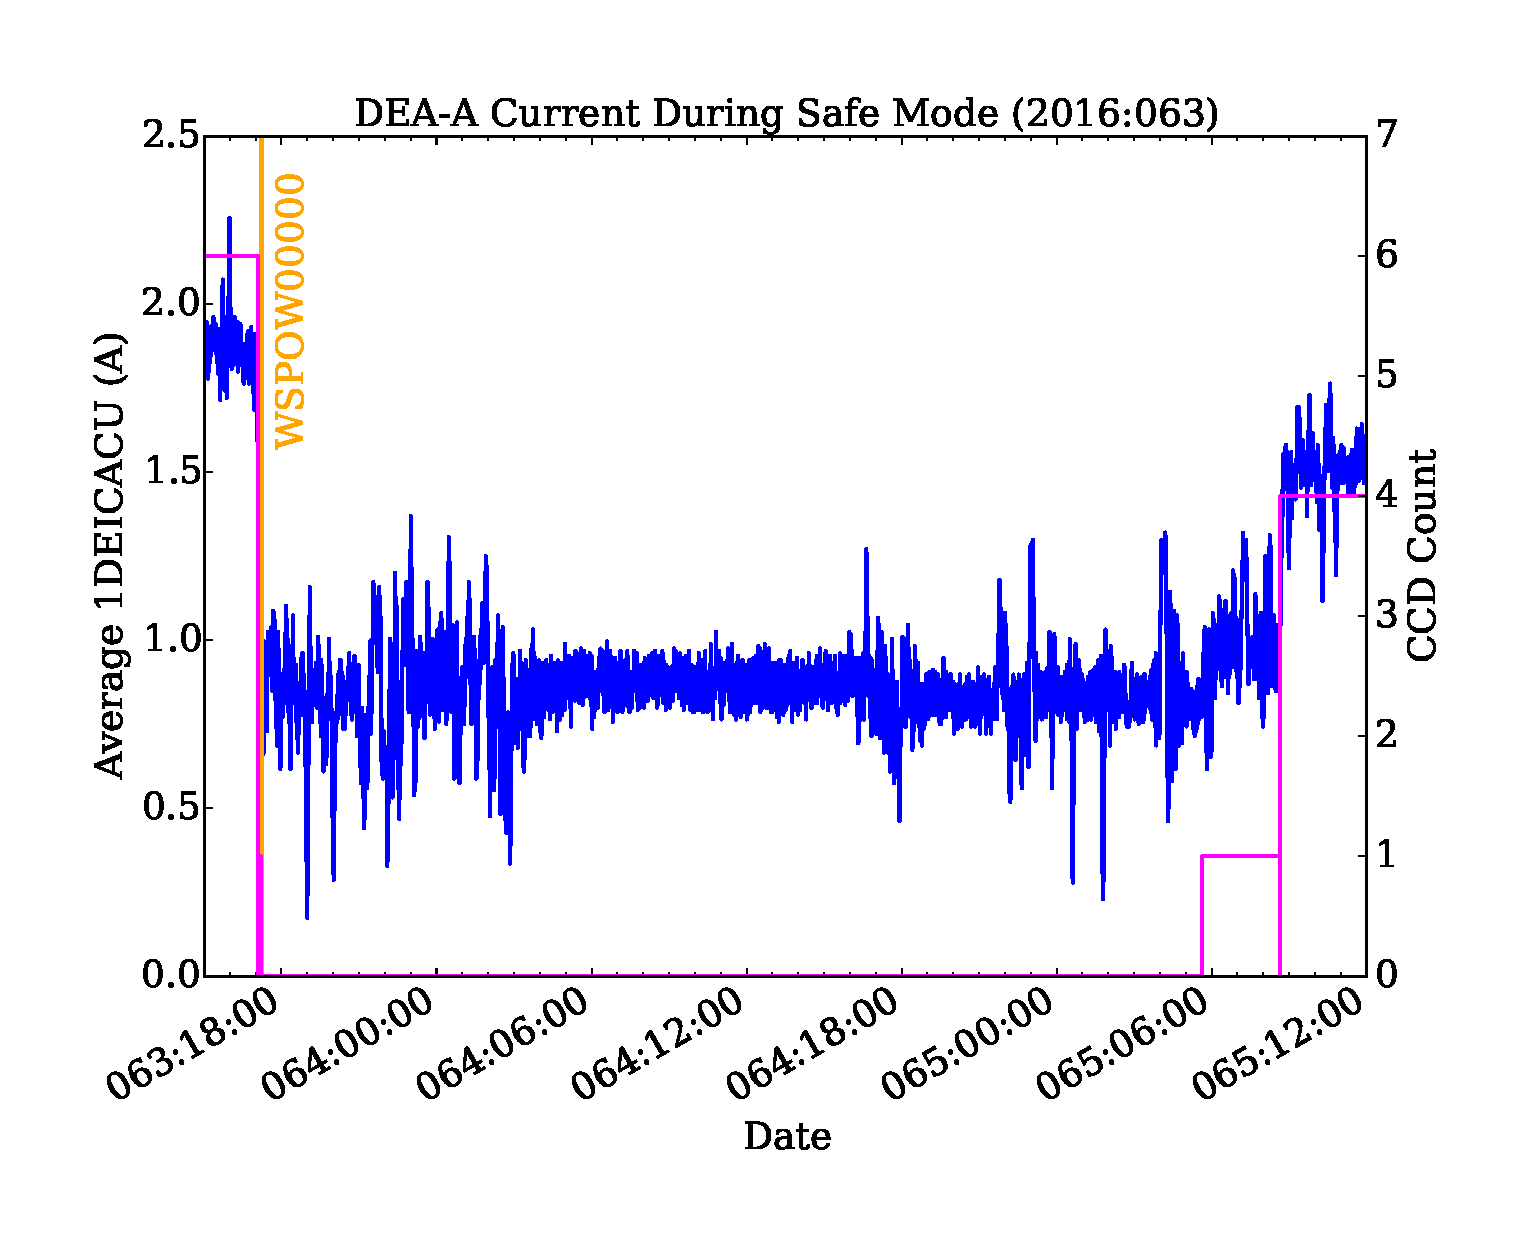
\includegraphics[width=1.2\textwidth]{deaa_on_test_vid_fig2.eps}
\caption{Average behavior of 1DEICACU during a safe mode. All video boards
are powered off after the issuing of the WSPOW00000 command, which is marked by
the orange line in the plot.}
\end{center}
\end{figure}
\end{landscape}

\begin{landscape}
\begin{figure}
\begin{center}
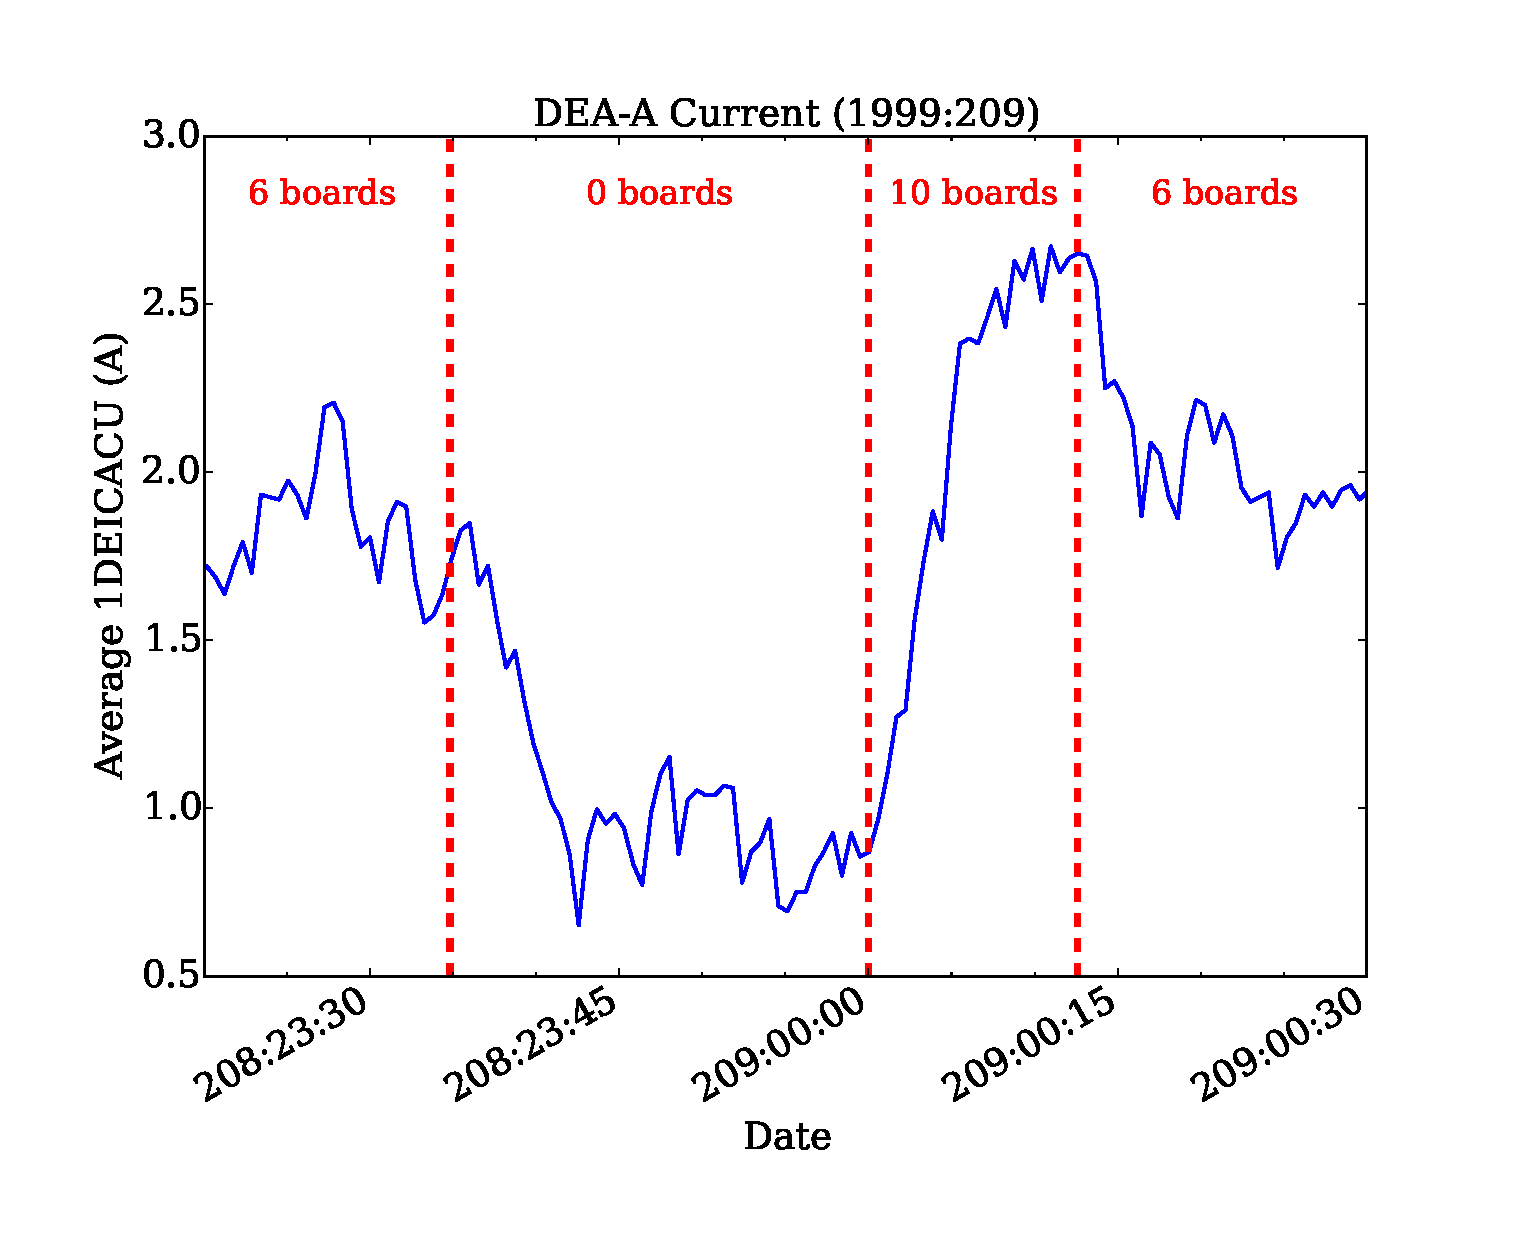
\includegraphics[width=1.2\textwidth]{deaa_on_test_vid_fig3.eps}
\caption{Average behavior of 1DEICACU with different numbers of video boards
powered on.}
\end{center}
\end{figure}
\end{landscape}

%\newpage\
%\vspace{0.4\textheight}
%\bc This page is intentionally blank \ec

\newcommand{\tablecaptiontext}{TURN ON DEA A AND TEST VIDEO BOARDS}
\documentclass[11pt]{article}

\usepackage{lscape,color}
\usepackage{graphicx}

\topmargin -0.75truein
\oddsidemargin -0.4truein
\textheight 9.25truein
\textwidth 6.7truein
\hbadness=10001
\hfuzz=200pt


\begin{document}
%\input dspace12.tex
%\input pstricks.tex
%\input psfig
\newcommand{\be}{\begin{enumerate}}
\newcommand{\ee}{\end{enumerate}}
\newcommand{\bc}{\begin{center}}
\newcommand{\ec}{\end{center}}
\newcommand{\bi}{\begin{itemize}}
\newcommand{\ei}{\end{itemize}}
\newcommand{\bd}{\begin{description}}
\newcommand{\ed}{\end{description}}
\newcommand{\bt}{\begin{tabbing}}
\newcommand{\et}{\end{tabbing}}
\newcommand{\eg}{{\it e.g.~}}
\newcommand{\ie}{{\it i.e.~}}
\newcommand{\ul}{\underline}
\newcommand{\axaf}{{\em AXAF}}
\def\la{\hbox{\rlap{$<$}\lower0.5ex\hbox{$\sim$}\ }}


\large
%\vspace*{-0.5in}
\centerline {\bf 4.29\_V2.1 TURN ON DEA A AND TEST VIDEO BOARDS }
\vspace{0.25in}

\normalsize
\noindent{\it Last Revised: June 5, 2017}\\
\noindent{\bf Filename: deaa\_on\_test\_vid} \\


\noindent {\bf BRIEF FUNCTIONAL DESCRIPTION:} \\
\normalsize

This is a procedure which powers up the DEA side A, powers up all 10 video boards, and powers up all 6 FEPs. It then executes an ACIS-I bias-only science run and an ACIS-S bias-only science run in order to get calibrated housekeeping data from the video boards. It then powers down all video boards and FEPs. It should be safe to execute under any condition except a spacecraft power or thermal emergency.

\vspace{0.25in}
\noindent The sequence of actions for this procedure will be:
\be
\item Verify that DEA B is powered off and disabled (see Constraints/Cautions, below)
\vspace{-0.10in}
\item Enable and turn on DEA power supply side A
\vspace{-0.10in}
\item Verify that DEA B is still off
\vspace{-0.10in}
\item Verify that the DH heater is not powered from side A
\vspace{-0.10in}
\item Power up all 10 video boards
\vspace{-0.10in}
\item Execute two bias-only science runs to capture video housekeeping
\vspace{-0.10in}
\item Power down the 10 video boards and the 6 FEPs
\ee

\vspace{0.15in}
\normalsize
\noindent {\bf ASSUMED INSTRUMENT STATE:} \\
\normalsize
\be
\item Assumes that the PSMC has power from the spacecraft.
\vspace{-0.10in}
\item Assumes that DEA B is off.
\vspace{-0.10in}
\item Assumes that both sides of the DPA are on.
\vspace{-0.10in}
\item Assumes that the flight SW is running on the active BEP.
\ee
\vspace{0.1in}
%\vspace{0.25in}
\normalsize
\noindent {\bf SPECIAL INITIAL CONDITIONS:} \\
\normalsize
%The environment must be clean enough to allow opening of the valve. \\
%Assumes that \axaf\/ ISIM RCTU is powered on and in telemetry format 6. \\

%\vspace{0.25in}
\normalsize
\noindent {\bf OPERATIONAL CONSTRAINTS/CAUTIONS:} \\
\normalsize

In normal operations, only one side of the DEA should be powered on
(a) to prevent conflict for control of the focal plane temperature controller,
(b) to avoid excess current draw from the spacecraft, and (c) to avoid over-heating
within the PSMC.

The DEA power status is normally indicated by the values of the 1DEPSA and
1DEPSB flags, which should not both be 1 simultaneously.

The DEA input current monitors (1DEIC[AB]CU) are noisy.
To give an indication of what variation may be expected, figures 1 and 2
show the behavior of the A-side DEA current with a ten-sample running
average for two situations in which all video boards were powered down. Note that
when either side of the DEA is unpowered, the corresponding current monitor, 
1DEICACU for side A, or 1DEICBCU for side B, will be unreliable. They will read
16--18~A when unpowered, as of Telemetry Database (TDB) v14. This is expected and
not a problem.

After successful execution, {\em the FP temperature control will be unregulated,
and DEA interface A/D will be in low-resolution mode.}\\

\vspace{0.15in}
\normalsize
\noindent {\bf REFERENCES:} \\
\normalsize

\normalsize
\noindent {\bf CHANGE HISTORY:} \\
\normalsize

{\bf V2.0}
\begin{itemize}
\item Branched off from ``deaa\_on'' atomic procedure V2.2
\item Add commands to power video boards on and off
\item Add bias-only science runs
\end{itemize}

{\bf V2.1}
\begin{itemize}
\item Added a step to verify DEA-B is off at the beginning of the procedure
\item Added text regarding power status issues and expected current behavior to the Operational Constraints/Cautions section. Also updated the expected FP temperature control.
\item Removed language about what to do if the DPA is unpowered since we do not expect to run this procedure if that is the case.
\item Removed input current check for DEA B; added warning to text.
\item Corrected introduction to indicate that we will be powering down all video boards and all FEPs at the end
\item Corrected numbering in table: 5.2 $\rightarrow$ 6.2
\item Corrected number of FEPMAN\_POWEROFF messages in Step 6.1 of the table
\end{itemize}

\begin{landscape}
\begin{figure}
\begin{center}
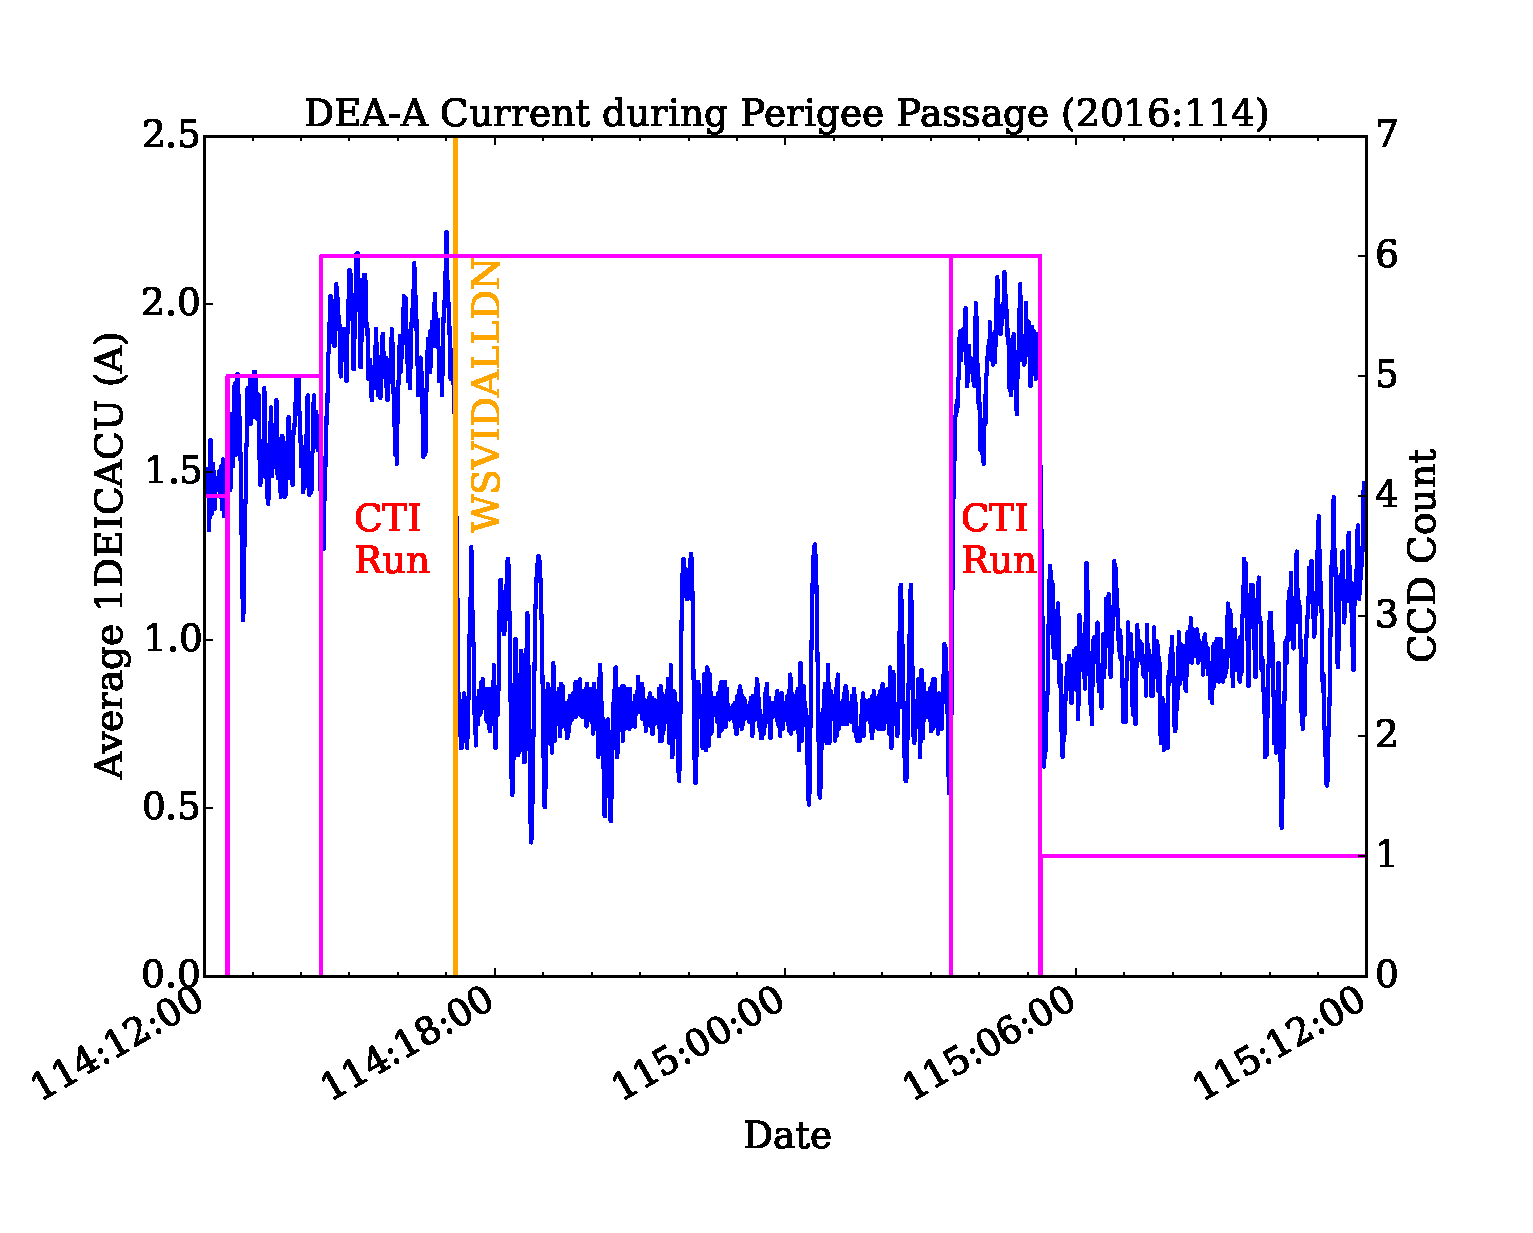
\includegraphics[width=1.2\textwidth]{deaa_on_test_vid_fig1.eps}
\caption{Average behavior of 1DEICACU during a perigee passage. All video boards
are powered off after the issuing of the WSVIDALLDN command, which is marked by
the orange line in the plot.}
\end{center}
\end{figure}
\end{landscape}

\begin{landscape}
\begin{figure}
\begin{center}
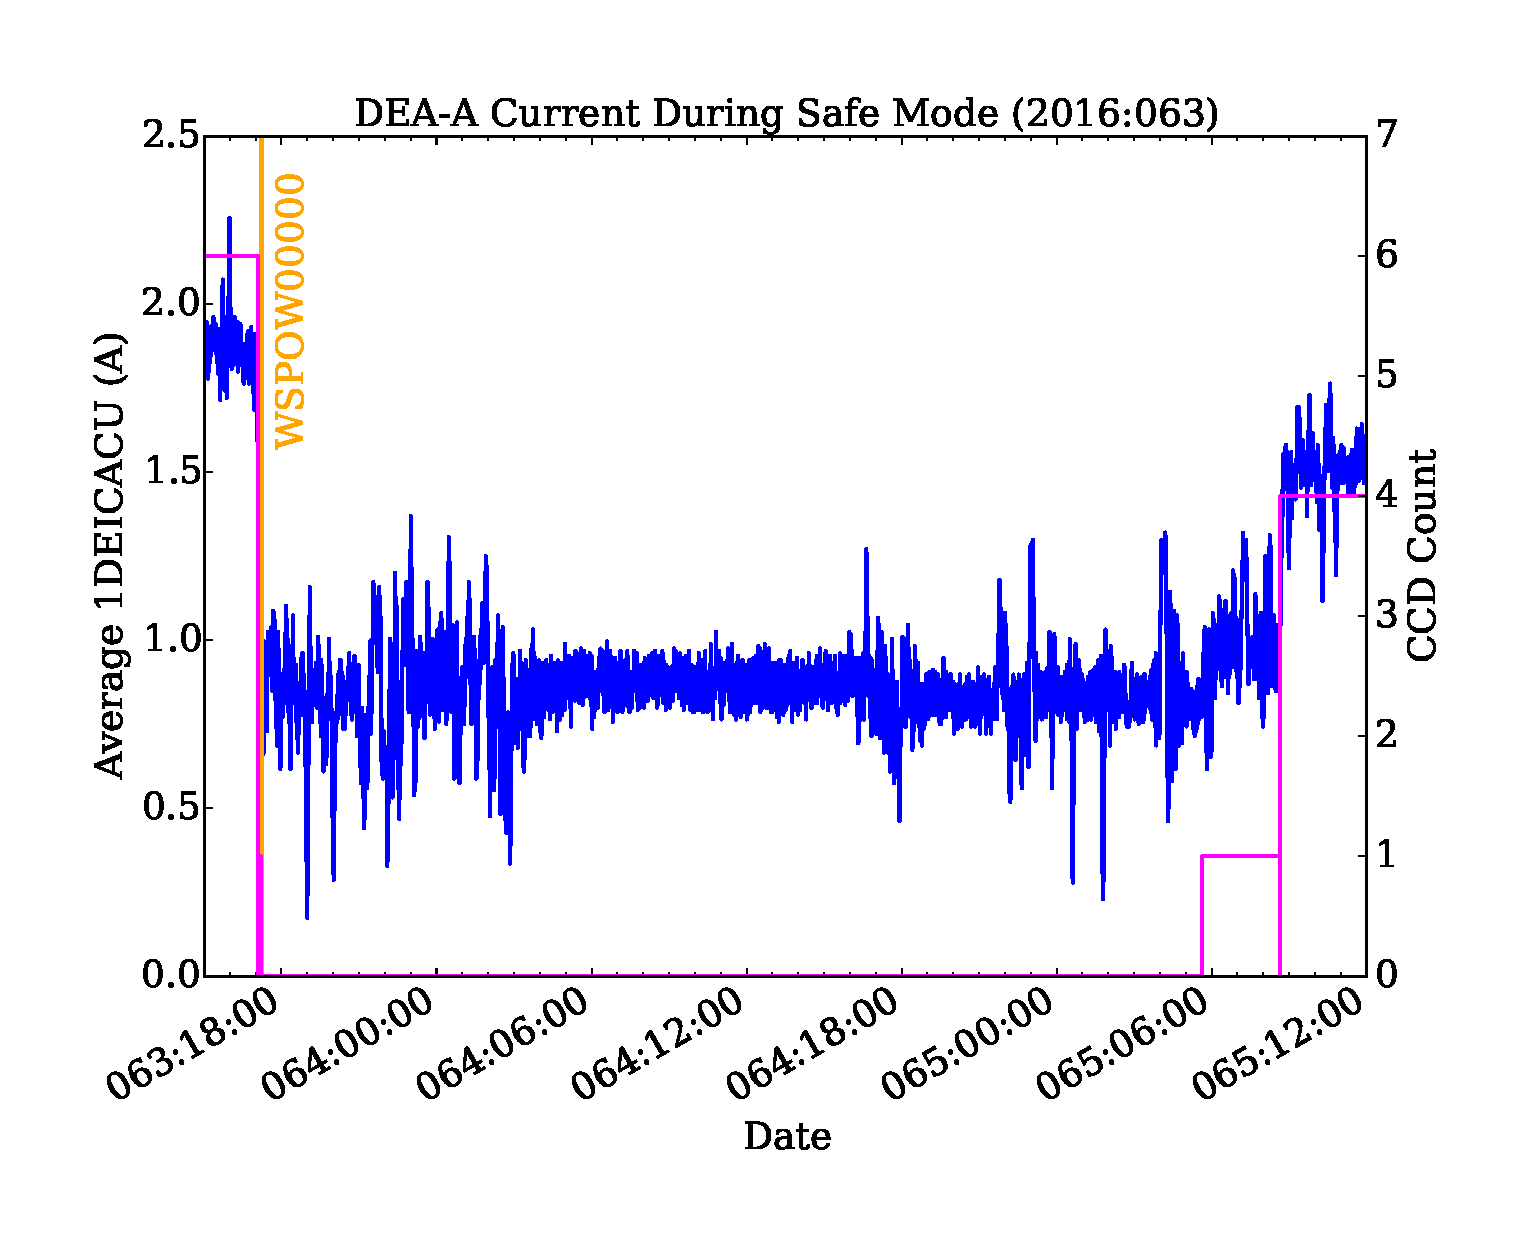
\includegraphics[width=1.2\textwidth]{deaa_on_test_vid_fig2.eps}
\caption{Average behavior of 1DEICACU during a safe mode. All video boards
are powered off after the issuing of the WSPOW00000 command, which is marked by
the orange line in the plot.}
\end{center}
\end{figure}
\end{landscape}

\begin{landscape}
\begin{figure}
\begin{center}
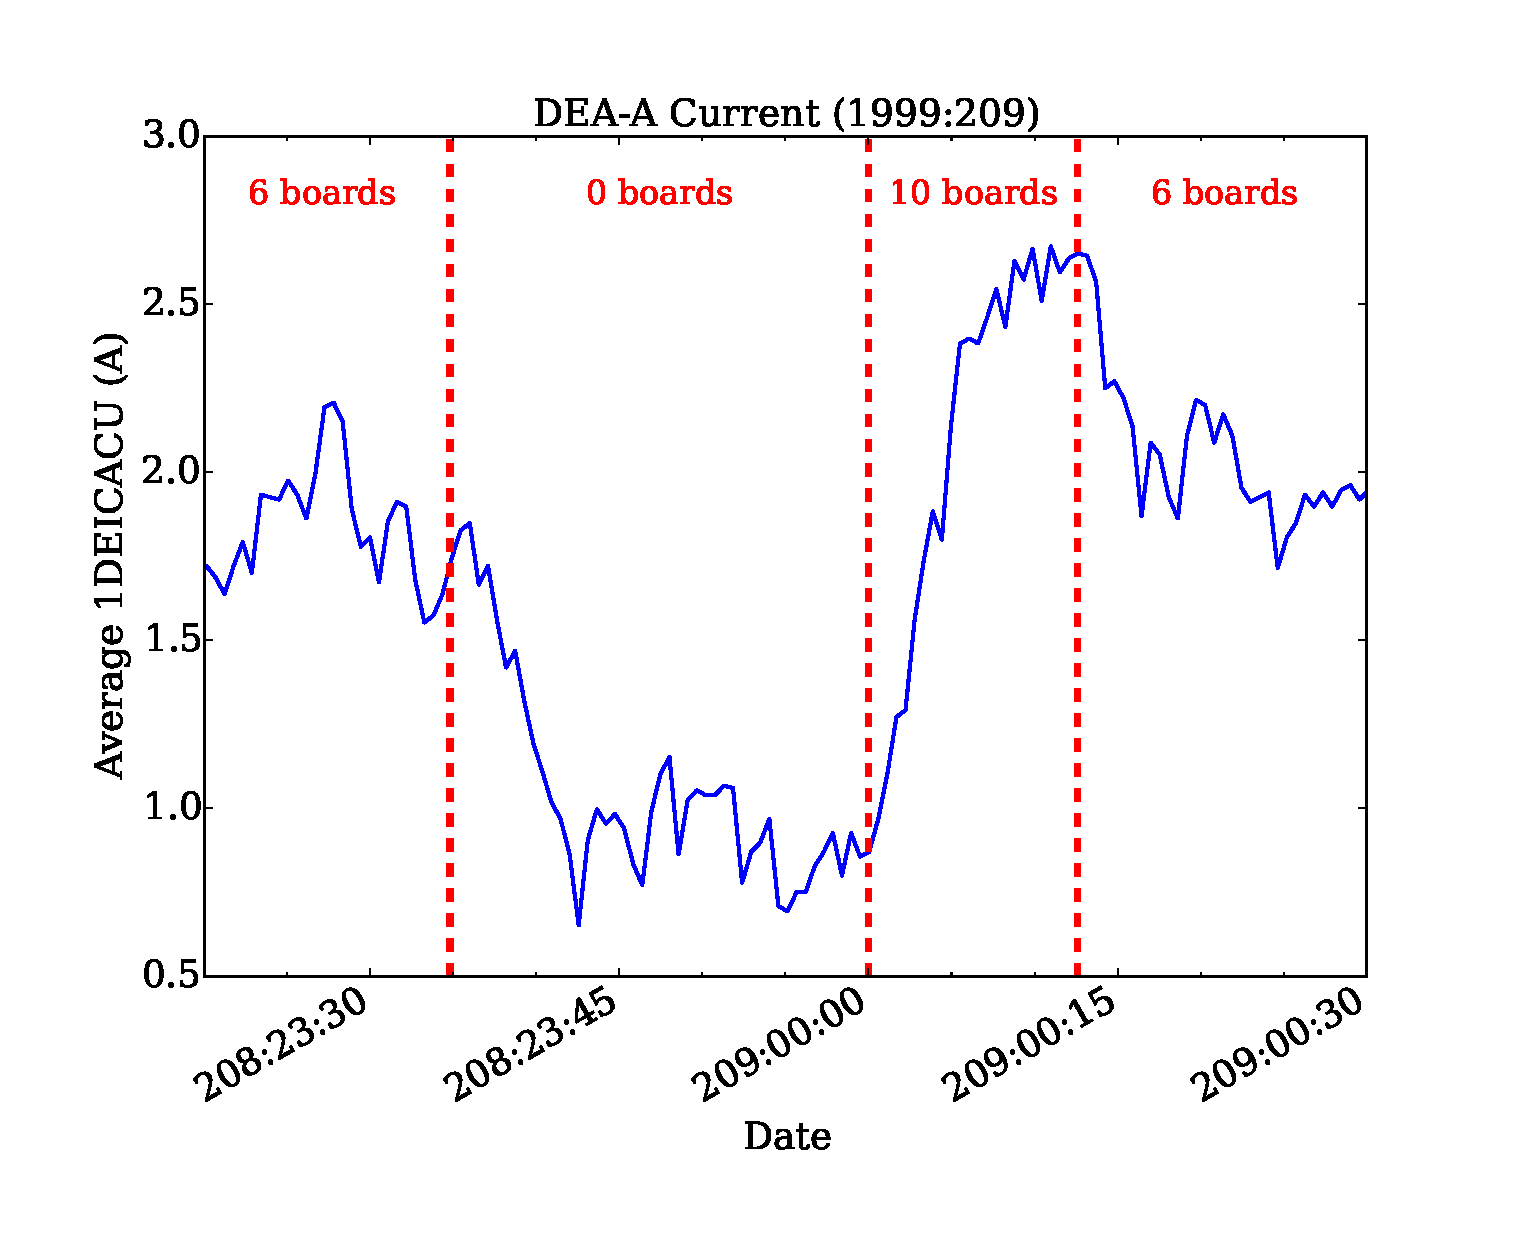
\includegraphics[width=1.2\textwidth]{deaa_on_test_vid_fig3.eps}
\caption{Average behavior of 1DEICACU with different numbers of video boards
powered on.}
\end{center}
\end{figure}
\end{landscape}

%\newpage\
%\vspace{0.4\textheight}
%\bc This page is intentionally blank \ec

\newcommand{\tablecaptiontext}{TURN ON DEA A AND TEST VIDEO BOARDS}
\input{deaa_on_test_vid.tab}

\end{document}


\end{document}


\end{document}


\end{document}
